%% 4. 「技術研究報告」
\documentclass[technicalreport]{ieicej}

\bibliographystyle{ieeetr}
%\usepackage{graphicx}
%\usepackage{latexsym}
\usepackage[dvipdfmx]{color}
\usepackage[dvipdfmx]{graphicx}
\usepackage{amsmath,amssymb,amsfonts}
%\usepackage{cite}
%\usepackage[psamsfonts]{amssymb}

\jtitle{フェージング環境におけるプライマリユーザ信号の時間的変化\\を考慮したデータベース精度向上法の検討}
\jsubtitle{}
\etitle{Accuracy Improvement for Spectrum Database considering\\Primary Signal in Time Domain Under Fading Environment}
\esubtitle{}
\authorlist{%
 \authorentry[wang\noexpand\noexpand\noexpand\_h@awcc.uec.ac.jp]{王\,\,\,\,\,\,昊}{Hao WANG}{awcc}% <= 記述しないとエラーになります
 \authorentry[k\noexpand\noexpand\noexpand\_sato@awcc.uec.ac.jp]{佐藤 光哉}{Koya SATO}{awcc}
 \authorentry[fujii@awcc.uec.ac.jp]{藤井 威生}{Takeo FUJII}{awcc}
}
\affiliate[awcc]{電気通信大学 先端ワイヤレス・コミュニケーション研究センター\\〒182-8585 東京都調布市調布ケ丘1丁目5-1}{Advanced Wireless and Communication research Center, The University of Electro-Communications,\\ 1-5-1 Chofugaoka, Chofu, Tokyo 182-8585, Japan}
%\affiliate[所属ラベル]{和文勤務先\\ 連絡先住所}{英文勤務先\\ 英文連絡先住所}
%\affiliate[所属ラベル]{和文勤務先\\ 連絡先住所}{英文勤務先\\ 英文連絡先住所}

\begin{document}
\begin{jabstract}
%和文あらまし
 コグニティブ無線を用いた周波数共用において,周波数の二次利用者(SU: Secondary User)は既存の周波数割り当てユーザ(PU: Primary User)への干渉を回避する必要がある.その中で自身の通信品質を確保するためには,正確な電波環境推定技術が重要である.現在,実用的な電波環境推定技術として電波環境データベースに注目を集めている.SUはデータベースに予め保存されるPUからの受信電力値に関する空間的な分布といった情報を取得することにより電波環境認識を行う.これまで車載無線機やスマートフォンといった移動端末が観測した膨大な電波環境情報から各位置における周波数の利用状況を高精度に構築される電波環境データベースが提案されている
テレビ帯域を対象とした実証実験により,従来の距離減衰モデルに基づく手法と比較してPUの平均受信電力値の空間的な分布を精度良く推定できることを明らかにしている.しかし,無線LANのように観測期間内に状態遷移する可能性のあるシステムについては,最終的な平均結果とON状態のみを抽出した平均受信電力値に差が生じる恐れがあった.
そこで本研究では,観測期間内にPUの通信状態が遷移する場合の電波環境データベースの構築について検討を行う.1回の観測期間内での受信電力に関する分布変化を検出することにより,PUの通信状態の遷移点を検出するアルゴリズムを提案する.検出した遷移点を用いて、通信を行なっている状態のみの受信電力値の取り出しが可能となり,PUが通信を行なっている状態での平均受信信号電力値を精度良く推定できる.本稿では特に,有効期間の検出に焦点を当てたシミュレーション評価を行ない,その有効性を示す.


\end{jabstract}
\begin{jkeyword}
%和文キーワード
コグニティブ無線,電波環境データベース,スペクトラムセンシング,遷移点検出
\end{jkeyword}
\begin{eabstract}
%英文アブストラクト
In order to improve spectrum utilization efficiency of Cognitive Radio (CR) systems, it is important for Secondary User (SU) to get knowledge about Primary User(PU)’s behavior when SU exploits opportunity to access spectrum. Radio Environment Database has recently been proposed to provide information about PU. Traditional advanced spectrum database constructed based on spectrum sensing method assumes that the transmit status of PU is always ON for updating the database information. However, it is not appropriate for recognizing in realistic environment because most of wireless systems does not always send the signal. In this paper, we propose a transition detection method using weighted cooperative sensing to construct a spectrum database for storing the power of PU obtained from sensor nodes. In the proposed method, the database gathers the information from sensor nodes and provides the previously stored information to generate the weight coefficient at the spectrum shared SUs. Then, we use a weighted cooperative sensing method to make a transition detection of PU behavior. Simulation results show that the proposed method can achieve a higher transition detection precision and the difference between the estimated transition point and the real transition point is smaller than the individual sensing.  
\end{eabstract}
\begin{ekeyword}
%英文キーワード
Cognitive Radio, Radio Environment Database, Spectrum Sensing, Energy Detection,Transition point Detection
\end{ekeyword}
\maketitle

\section{研究背景}

\begin{figure}[t]
  \centering
  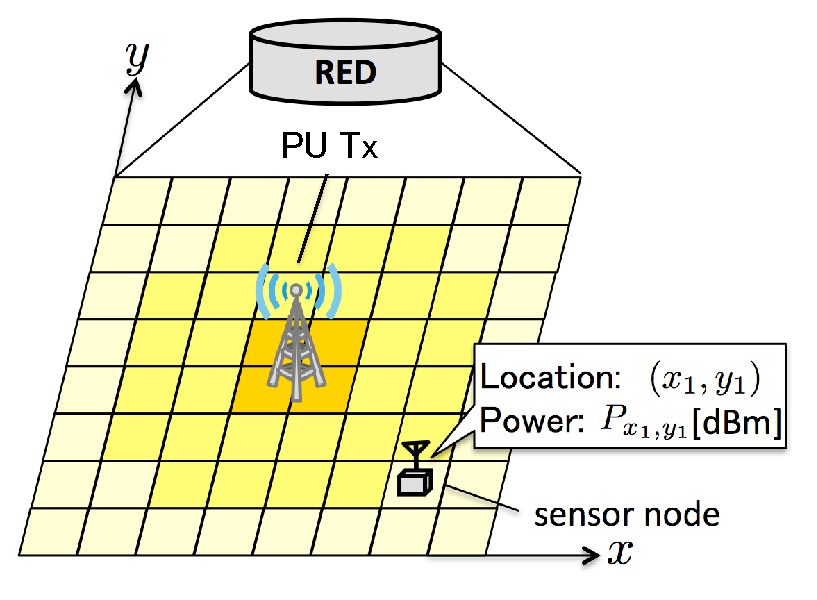
\includegraphics[width=0.8\hsize,clip]{database.eps}
  \caption{電波環境データベース}
  \label{databse}
\end{figure}



\section{システムモデル}
\label{sec:model}
\begin{figure}[t]
\centering
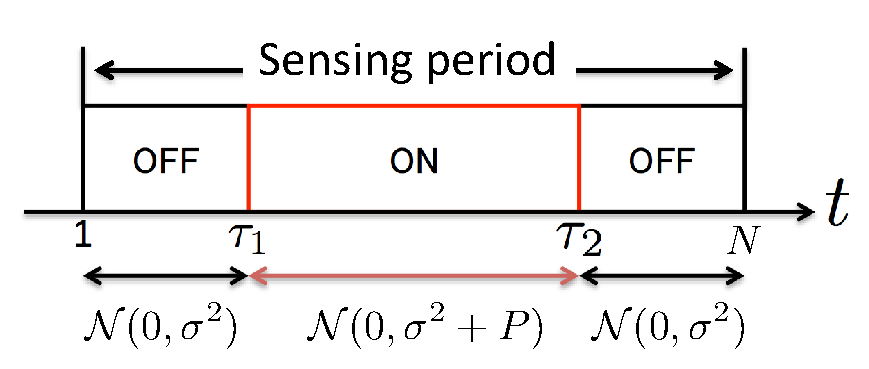
\includegraphics[width=0.8\hsize,clip]{systemmodel.eps}
\caption{\normalsize{システムモデル}}
\label{systemmodel}
\end{figure}


\section{遷移点検出法}
\label{sec:transition}

\subsection{CUSUMアルゴリズム($\simga^2$既知,)}

\subsection{GLRアルゴリズム}

\section{フェージング環境における遷移点検出による有効期間検出}
\label{sec:propose}


\section{シミュレーション結果及び性能評価}
\label{sec:result}

\section{結論}
\label{sec:conclusion}

\ack

本研究はJSPS科研費15H04004,15H04010の助成を受けたものです.


\bibliographystyle{sieicej}
%\bibliography{myrefs}
 \begin{thebibliography}{10}
\bibitem{ref:Cisco}Cisco, ``Cisco Visual Networking Index: Global Mobile Data Traffic Forecast Update, 2014–2019,''Cisco White Paper.
\bibitem{ref:FCC}Federal Communications Commission, ``Spectrum policy task force report,fcc 02-155,'' Nov. 2002.
\bibitem{ref:mitola}J. Mitola III and G. Q. Maguire, Jr., ``Cognitive radio: making software radios more personal,'' IEEE Personal Communications, vol. 6, no. 4, pp. 13–18, Aug. 1999.
\bibitem{ref:Haykin} S. Haykin, ``Cognitive radio: Brain-empowered wireless communications,'' {\it IEEE J.Selected Areas Commun.},vol. 23, no. 2, pp. 201 - 220, Feb. 2005.
\bibitem{ref:fujii_Database} K. Sato, M. Kitamura, K. Inage, and T. Fujii, ``Measurement-based spectrum database for flexible spectrum management,'' IEICE Trans. Commun., vol.E98-B, no.10, pp.2004-2013, Oct. 2015.
\bibitem{ref:ON1}G. Zhou, J. Wu, K. Sohraby, ``Cooperative Spectrum Sensing with a Progressive MAP Detection Algorithm,'' Proc. GLOBECOM, pp.1-5, Dec. 2011.
\bibitem{ref:ON2}Y. Pei, Y. Liang, K.C.Teh, K. H. Li, ``Sensing-throughput tradeoff for cognitive radio networks: A multiple-channel sceario,'' Proc. IEEE PIMRC, pp.1257-1261, 13-16 Sept. 2009.
\bibitem{ref:quickest}L.Lai, Y.Fan, and H.V.Poor, ``Quickest Detection in Cognitive Radio: A Sequential Change Detection Framework,'' Proc. IEEE Globecom, Dec. 2008.
\bibitem{ref:overlay}Vameghestahbanati, M. and Mir, H.S. and El-Tarhuni, M., `` An overlay architecture for cognitive radio systems,'' Proc. IEEE ICCSPA, pp.1-4, Feb. 2014.
\bibitem{ref:underlay}H. Hu and Q. Zhu, ``Dynamic Spectrum Access in Underlay Cognitive Radio System with SINR Constraints,'' Proc. IEEE WiCompp. 1-4, Sept. 2009.
\bibitem{ref:fcc}Federal Communications Commission, SECOND MEMORANDUM OPINION AND ORDER, Sept. 2010.
\bibitem{ref:google}Google, ``Spectrum database.'' http://www.google.org/spec\\trum/whitespace/, accessed Jan. 15. 2016.
\bibitem{ref:ED}T. Yucek and H. Arslan, ``A survey of spectrum sensing algorithms for cognitive radio applications,'' IEEE {\it Communications Surveys Tutorials}, vol. 11, no. 1, pp. 116-130, 2009.
\bibitem{ref:CUSUM}E. Page, ``Continuous inspection schemes,'' {\it Biometrika}, vol. 41, pp. 100-115, 1954.
\bibitem{ref:GLR}G. Lorden, ``Procedures for reacting to a change in distribution,'' {\it Annals of Mathematical Statistics}, vol. 42, no. 6, pp. 1897-1908, 1971.  
\bibitem{ref:threshold_cusum}G. Lorden, ``ON excess over the boundary,'' {\it Annals of Mathematical Statistics}, vol. 41, pp.520-527, Apr. 1970.
\bibitem{ref:threshold_GLR}G. Lorden, ``Open-ended tests for Koopman-Darmois families,'' {\it Annals of Statistics}, vol. 1, no. 4, pp. 520-527, Apr. 1970.
 \end{thebibliography}
 
\end{document}
